% Auto-generated by the analysis pipeline — do not edit
% y > 0: Overreacts  |  y < 0: Underreacts
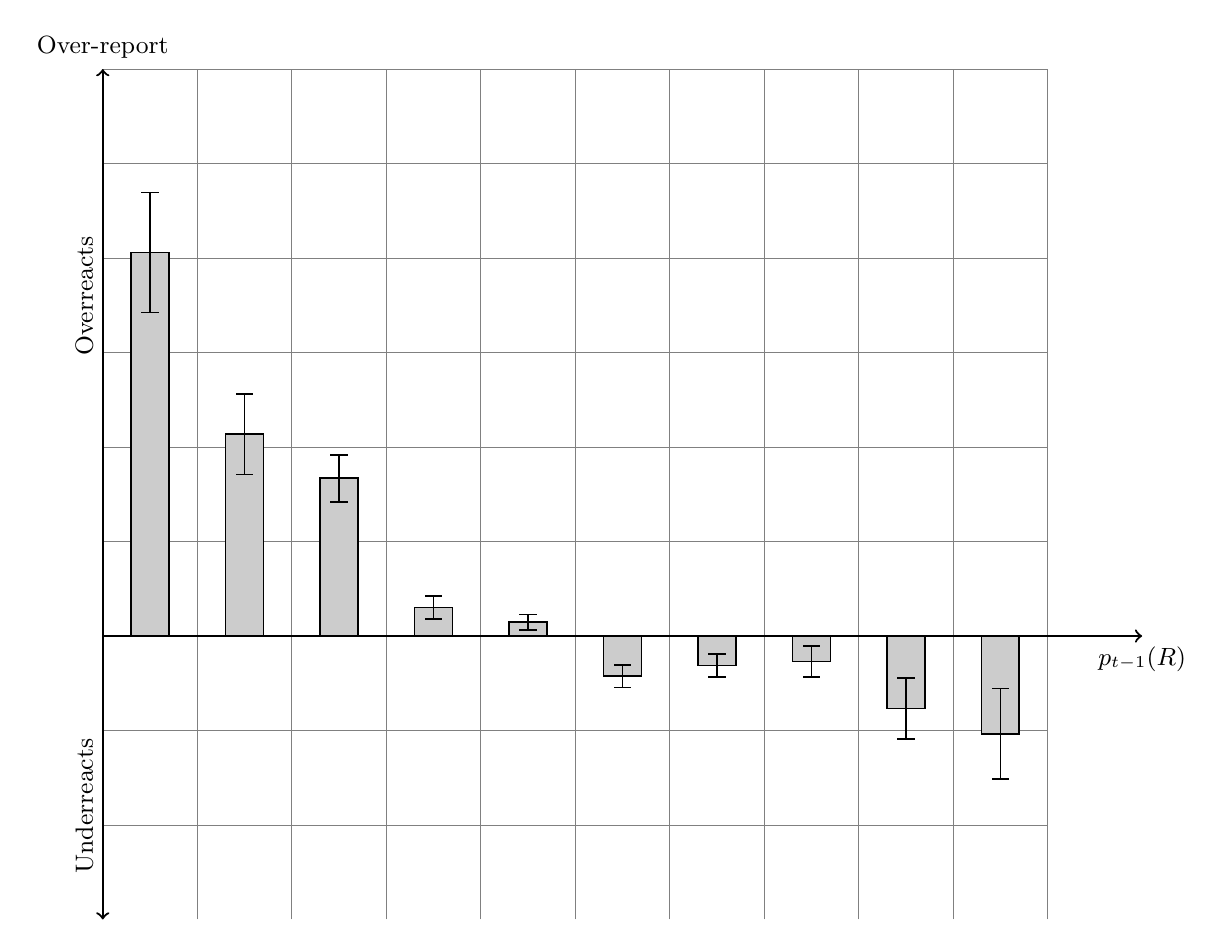
\begin{tikzpicture}[scale=12]
\draw[help lines,step=0.1] (0,-0.3) grid (1,0.6);
\filldraw[opaque,white!80!black] (0.03,0) rectangle (0.07,0.4058);
\draw[line width=0.6] (0.03,0) rectangle (0.07,0.4058);
\draw[line width=0.6,|-|] (0.05,0.3416) -- (0.05,0.4701);
\filldraw[opaque,white!80!black] (0.13,0) rectangle (0.17,0.2135);
\draw[line width=0.6] (0.13,0) rectangle (0.17,0.2135);
\draw[line width=0.6,|-|] (0.15,0.1700) -- (0.15,0.2570);
\filldraw[opaque,white!80!black] (0.23,0) rectangle (0.27,0.1669);
\draw[line width=0.6] (0.23,0) rectangle (0.27,0.1669);
\draw[line width=0.6,|-|] (0.25,0.1412) -- (0.25,0.1926);
\filldraw[opaque,white!80!black] (0.33,0) rectangle (0.37,0.0302);
\draw[line width=0.6] (0.33,0) rectangle (0.37,0.0302);
\draw[line width=0.6,|-|] (0.35,0.0173) -- (0.35,0.0431);
\filldraw[opaque,white!80!black] (0.43,0) rectangle (0.47,0.0147);
\draw[line width=0.6] (0.43,0) rectangle (0.47,0.0147);
\draw[line width=0.6,|-|] (0.45,0.0057) -- (0.45,0.0237);
\filldraw[opaque,white!80!black] (0.53,0) rectangle (0.57,-0.0426);
\draw[line width=0.6] (0.53,0) rectangle (0.57,-0.0426);
\draw[line width=0.6,|-|] (0.55,-0.0553) -- (0.55,-0.0299);
\filldraw[opaque,white!80!black] (0.63,0) rectangle (0.67,-0.0311);
\draw[line width=0.6] (0.63,0) rectangle (0.67,-0.0311);
\draw[line width=0.6,|-|] (0.65,-0.0440) -- (0.65,-0.0182);
\filldraw[opaque,white!80!black] (0.73,0) rectangle (0.77,-0.0269);
\draw[line width=0.6] (0.73,0) rectangle (0.77,-0.0269);
\draw[line width=0.6,|-|] (0.75,-0.0443) -- (0.75,-0.0095);
\filldraw[opaque,white!80!black] (0.83,0) rectangle (0.87,-0.0767);
\draw[line width=0.6] (0.83,0) rectangle (0.87,-0.0767);
\draw[line width=0.6,|-|] (0.85,-0.1102) -- (0.85,-0.0432);
\filldraw[opaque,white!80!black] (0.93,0) rectangle (0.97,-0.1034);
\draw[line width=0.6] (0.93,0) rectangle (0.97,-0.1034);
\draw[line width=0.6,|-|] (0.95,-0.1522) -- (0.95,-0.0547);
\draw[line width=0.8,->]  (0,0) -- (1.1,0) node[below] {\small{$p_{t-1}(R)$}};
\draw[line width=0.8,<->] (0,-0.3) -- (0,0.6) node[above] {\small{Over-report}};
\draw (0,0.36) node[above,rotate=90] {\small{Overreacts}};
\draw (0,-0.18) node[above,rotate=90] {\small{Underreacts}};
% ADD THEORY CURVE BELOW
\end{tikzpicture}
